\documentclass[11pt]{article}
\usepackage{amsmath}
\usepackage{booktabs}
\usepackage{geometry}
\usepackage{graphicx}
\usepackage[round]{natbib}
\geometry{margin=1in}
\bibliographystyle{plainnat}

\title{Standalone Methods Draft:\\Functional Synaptic Interactions and Inhibitory Circuitry of the PreB\"otzinger Complex in the Rhythmic Slice}
\author{}
\date{}

\begin{document}

\maketitle

\section{Methods}

\subsection{Animals, slice preparation, and cell targeting}
All animal procedures were approved by the Animal Care and Use Committee of the National Institute of Neurological Disorders and Stroke (Animal Study Proposal 1154--21). Experiments were performed on neonatal (postnatal day 3--8) mice of either sex in rhythmically active medullary slice preparations, as described previously for genetically identified preB\"otC neurons in reduced respiratory preparations \citep{koizumi2013structural,ausborn2018organization}. Excitatory neurons were targeted in Slc17a6-Cre;Rosa-tdTomato mice (referred to here as VgluT2-tdTomato mice), and inhibitory neurons were targeted in VGAT-Cre;Rosa-tdTomato mice (VGAT-tdTomato mice). TdTomato-positive neurons in the preB\"otC were identified by live fluorescence imaging and targeted for whole-cell recording.

Rhythmically active slices (300--400~$\mu$m) were superfused at 4~ml/min with artificial cerebrospinal fluid containing (in mM): 124 NaCl, 25 NaHCO$_3$, 3 KCl, 1.5 CaCl$_2$, 1.0 MgSO$_4$, 0.5 NaH$_2$PO$_4$, and 30 D-glucose, equilibrated with 95\% O$_2$/5\% CO$_2$ (pH 7.35--7.40, 27$^\circ$C). Rhythmic respiratory activity was maintained by elevating extracellular K$^+$ to 8--9~mM. Inspiratory motor output was monitored from hypoglossal (XII) rootlets with suction electrodes, amplified 50{,}000--100{,}000$\times$, band-pass filtered at 0.3--2~kHz, and digitized at 10~kHz.

The slice experiments were technically more challenging than the rat respiratory preparations used in many earlier studies. In particular, mouse XII rootlets were often delicate, and the recorded inspiratory output was not always the large, stereotyped population burst routinely observed in rat slices. Depending on how many fibers were captured by the suction electrode, the integrated XII trace could reflect only a partial motor output and could be less stationary across the file. We therefore treated the XII recording primarily as a cycle-timing reference and used additional preprocessing safeguards when the rootlet signal alone was too weak or unstable for reliable phase detection.

Optical targeting was performed with a Leica TCS SP5 II MP upright microscope equipped with a 20$\times$ water-immersion objective (NA 1.0) and a Ti:Sapphire laser (800--880~nm) for two-photon fluorescence imaging. Whole-cell current-clamp and voltage-clamp recordings were obtained with a HEKA EPC-9 amplifier using borosilicate electrodes (4--6~M$\Omega$) filled with (in mM): 130 K-gluconate, 5 Na-gluconate, 3 NaCl, 10 HEPES, 4 Mg-ATP, 0.3 Na-GTP, and 4 sodium phosphocreatine, adjusted to pH~7.3 with KOH. Measured voltages were corrected for a $-10$~mV liquid-junction potential. Series resistance was compensated online by approximately 80\% and adjusted during the recording. Voltage-clamp recordings with obvious space-clamp failure were excluded before quantitative analysis.

\subsection{Recording inventory, acquisition modes, and acceptance screening}
The repository contains 59 analyzed slice recordings spanning four phenotype groups: VgluT2 inspiratory (VgluT2-I), VgluT2 expiratory (VgluT2-E), VGAT inspiratory (VGAT-I), and VGAT expiratory (VGAT-E). These files are recording-level analysis units rather than unique-cell counts, because some neurons contributed separate current-clamp (C) and voltage-clamp (V) recordings. Raw electrophysiological and XII signals were originally digitized at 10~kHz and then downsampled to 1~kHz for the exported analysis files used in this repository. This downsampling preserved the slower respiratory-cycle modulation, the stepwise command epochs, and the phase-binned current--voltage relationships used for conductance inference; reconstruction of the detailed spike waveform was not required for the analysis. Each exported trace contained four aligned columns: time, current channel, voltage channel, and integrated XII activity. In current clamp, the current and voltage channels corresponded to injected current and membrane potential, respectively; in voltage clamp, they corresponded to measured holding current and command voltage.

Because the slice recordings were more heterogeneous than the higher-quality data analyzed in the companion \textit{in situ} study of \citet{molkov2024inference}, we did not impose rigid file-level requirements such as at least three usable command steps or a prescribed current/voltage span. In this data set, criteria of that type would have discarded approximately two-thirds of the available slice recordings before any conductance-based quality control, largely for technical rather than biological reasons. Instead, we used an inclusive recording-level screen and then applied robust outlier filtering only after conductance reconstruction. The only hard acceptance criterion for inclusion in the population summaries was that the analyzed segment contain more than 25 detected XII cycles across the retained interval. This yielded 50 accepted recordings (27 current clamp, 23 voltage clamp): 20 VgluT2-I, 12 VGAT-I, 17 VGAT-E, and 1 VgluT2-E recording (Table~\ref{tab:inventory}). The accepted recording set corresponds to 31 neuron-level identifiers, so the $N$ values used in summary plots and tables refer to recordings, not unique cells. We retained current-clamp and voltage-clamp files as separate analysis units because mode-to-mode variability was comparable to cell-to-cell variability, while the two modes yielded qualitatively consistent conductance estimates.

\begin{table}[htbp]
\centering
\small
\caption{Recording inventory in the repository and after automated cycle-count screening. Counts refer to recordings, not unique neurons.}
\label{tab:inventory}
\begin{tabular}{lcccc}
\toprule
Population & Candidate files & Accepted files & Accepted C & Accepted V \\
\midrule
VgluT2-I & 23 & 20 & 12 & 8 \\
VgluT2-E & 2 & 1 & 1 & 0 \\
VGAT-I & 17 & 12 & 6 & 6 \\
VGAT-E & 17 & 17 & 8 & 9 \\
\midrule
Total & 59 & 50 & 27 & 23 \\
\bottomrule
\end{tabular}
\end{table}

The command protocols used for conductance inference consisted of piecewise-constant current steps in current clamp and piecewise-constant holding-voltage steps in voltage clamp (Figure~\ref{fig:protocol}). A representative current-clamp/voltage-clamp pair from the same VgluT2-I neuron is shown to make the stepped acquisition strategy explicit, because this feature is not obvious from the conductance-reconstruction figure alone. Across the retained stationary interval, the multiple command levels were not analyzed one step at a time; instead, samples from all usable steps were pooled within each respiratory phase bin so that the full recording collectively supplied the current--voltage spread needed for phase-specific regression.

\begin{figure}[htbp]
\centering
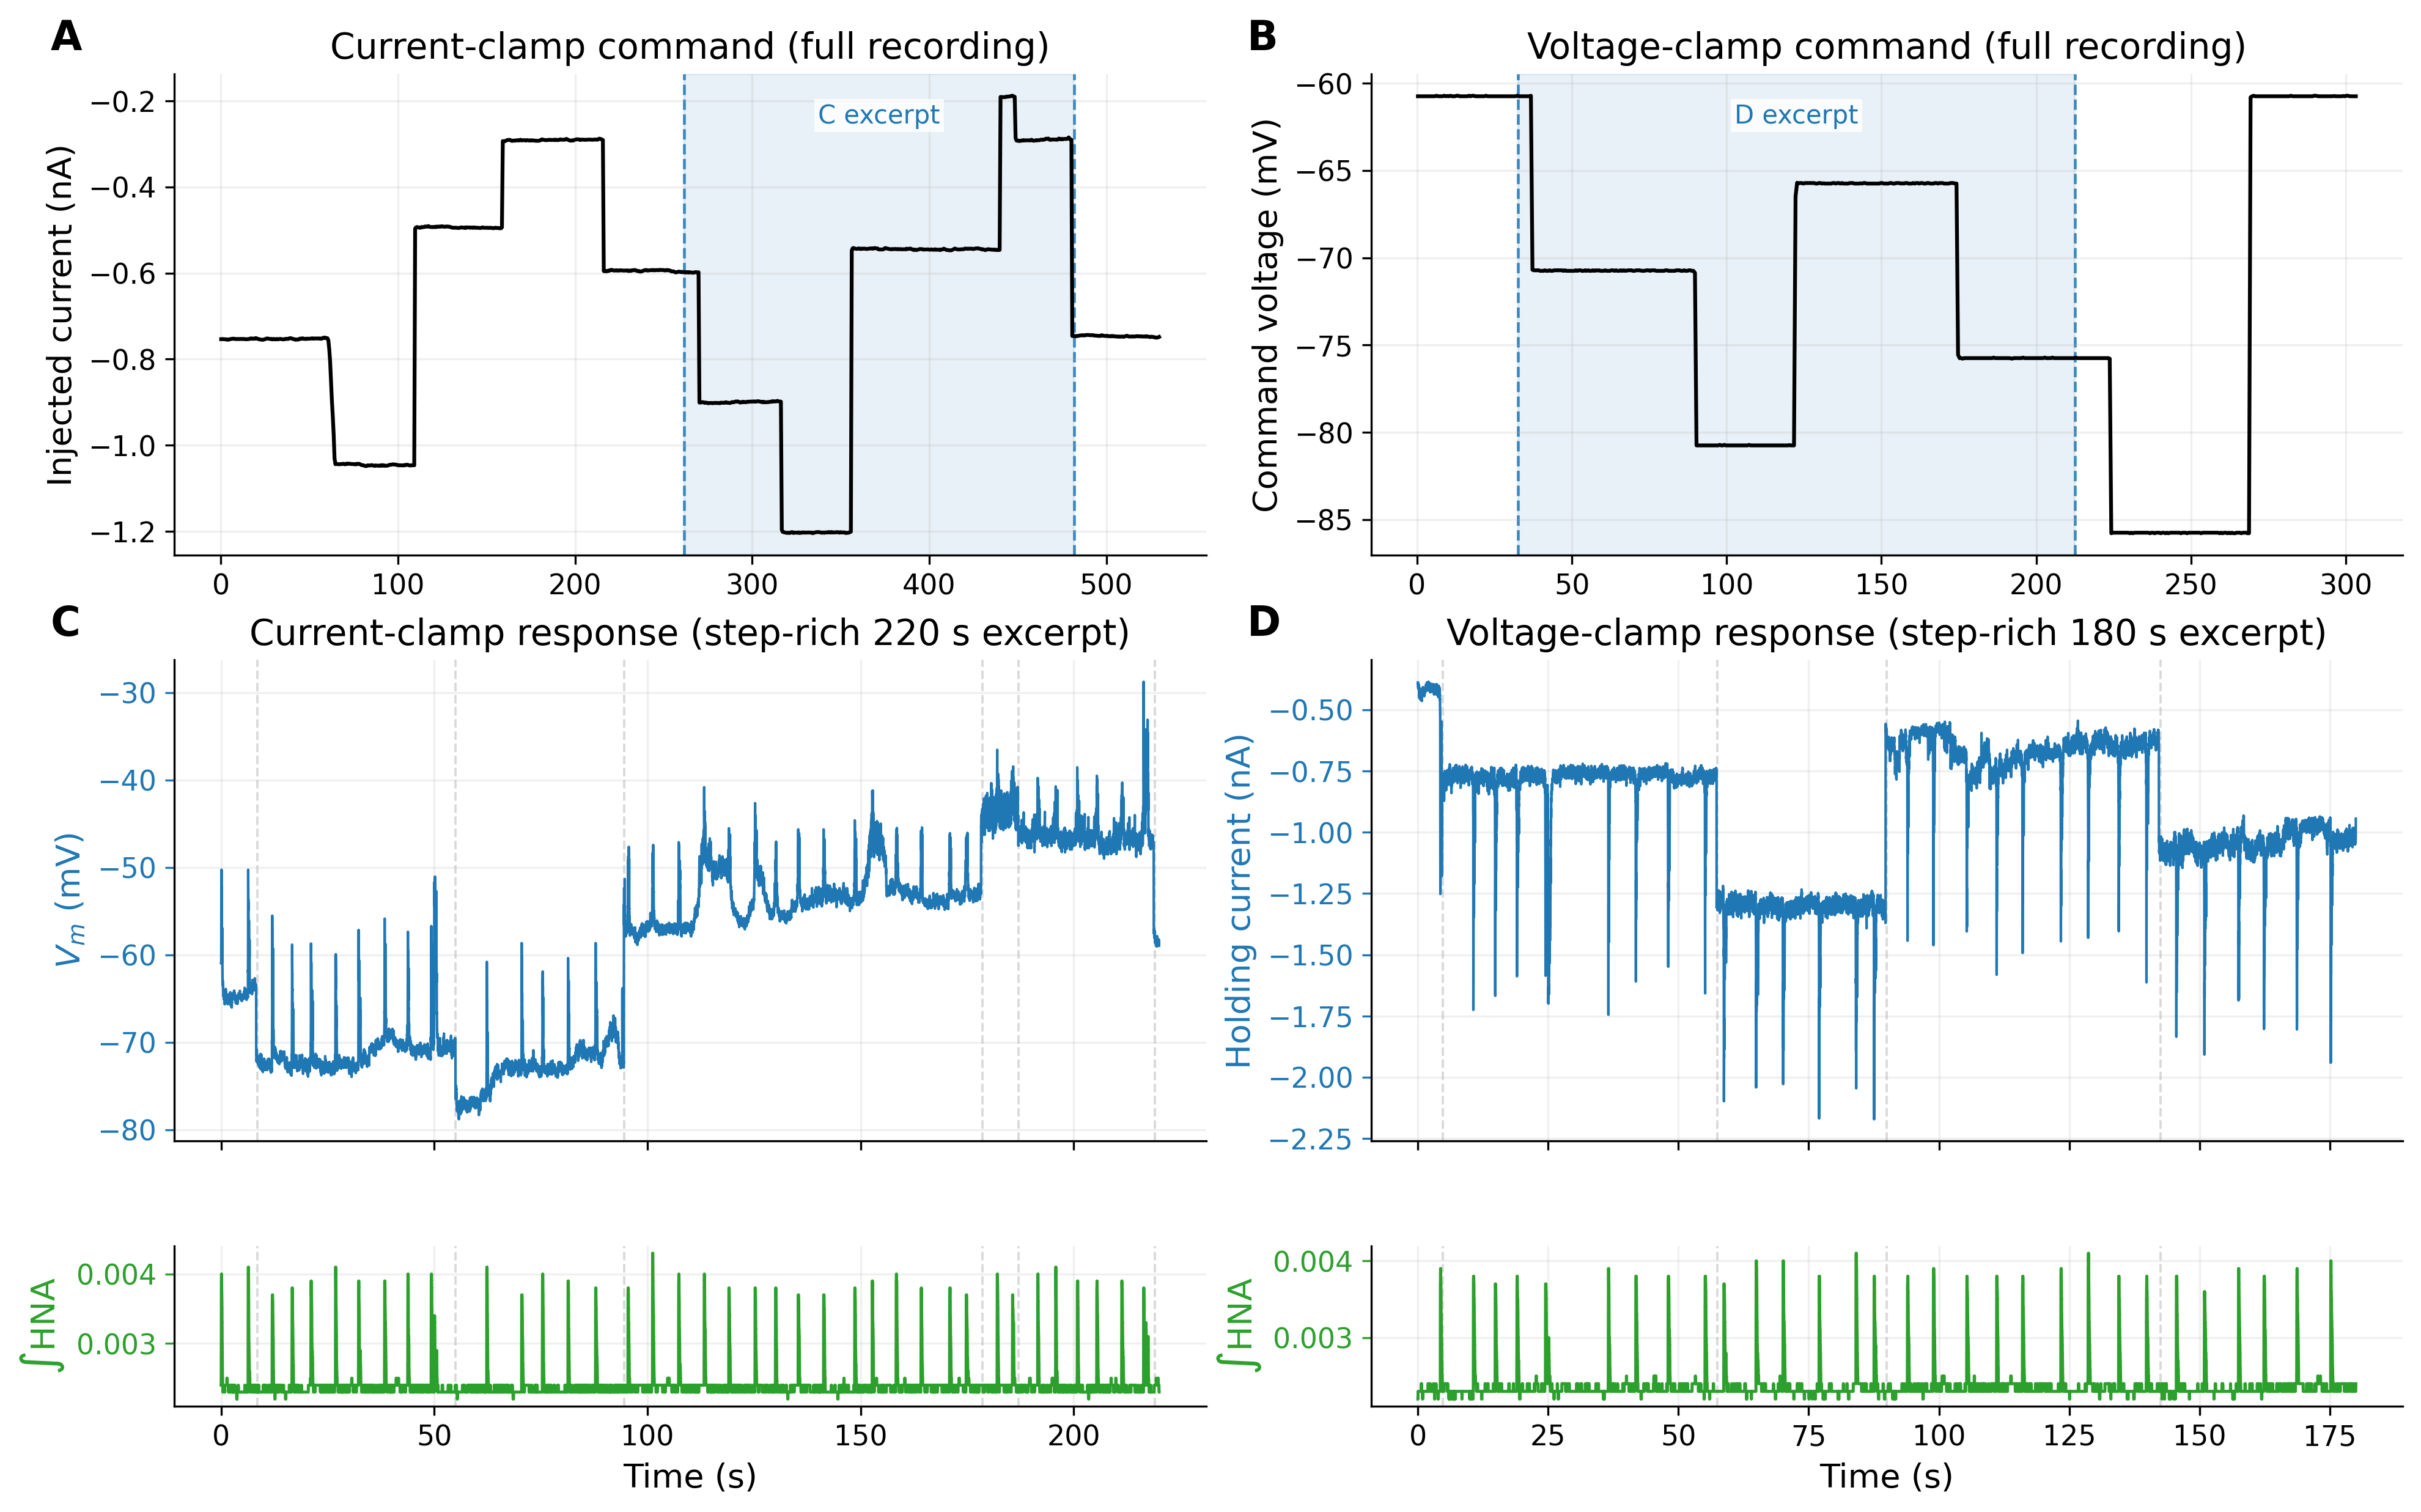
\includegraphics[width=\textwidth]{figures/method_protocol_steps.png}
\caption{Representative stepped acquisition protocols used for conductance inference. \textbf{A}, full current-clamp command trace for VgluT2-I-Cell2-C, shown after coarse median smoothing to highlight the piecewise-constant current injections; the blue shaded interval marks the segment expanded in panel~\textbf{C}. \textbf{B}, full voltage-clamp command trace for the matched recording VgluT2-I-Cell2-V; the blue shaded interval marks the segment expanded in panel~\textbf{D}. \textbf{C--D}, longer step-rich excerpts selected automatically from later portions of the same two recordings; the response channel is plotted in the upper lane (membrane potential in current clamp, holding current in voltage clamp) and the integrated XII reference is plotted separately in the lower lane. Gray dashed lines mark command transitions that fall inside the excerpt. The full command traces were used to sample a range of current--voltage operating points across many respiratory cycles.}
\label{fig:protocol}
\end{figure}

\subsection{Manual curation and preprocessing of analyzed segments}
Several recordings required limited manual curation before automated inference. The purpose of this step was to isolate the longest interval that was reasonably stationary in both the electrophysiological channels and the respiratory reference, rather than to select epochs with any particular conductance pattern. Files were therefore trimmed at the beginning when the recording was still stabilizing, at the end when rhythmicity or seal quality deteriorated, and, when instability was present at both ends, to the middle portion that remained acceptably stationary. Thus ``middle selection'' was implemented by defining start and end boundaries around a single contiguous interval rather than by stitching together disjoint fragments. In the current repository version, 6 accepted recordings used a non-zero starting offset and 6 used an explicit end truncation. These edits were intentionally conservative and were applied before any conductance estimates were calculated.

All signal processing was then automated. The current and voltage channels were median-filtered with a per-file half-width defined in the analysis configuration (default 25 samples, corresponding to a 51-sample window). Because the mouse XII rootlet signal was not always sufficiently robust on its own, the reference channel was optionally combined with the simultaneously recorded electrophysiological channel when the rootlet trace was too weak, noisy, or unstable to give reliable cycle onsets. In those cases, the reference channel was converted to a local z-score and linearly combined with a local z-score of the membrane-potential channel (current clamp) or the current channel (voltage clamp):
\begin{equation}
p_{\mathrm{mix}}(t) = z\!\left[p(t)\right] + s\,z\!\left[y(t)\right],
\end{equation}
where $p(t)$ is the integrated XII signal, $y(t)$ is the auxiliary electrophysiological channel, and $s=\pm 1$ was chosen empirically to align the sign of the auxiliary signal with inspiratory onset. Local means and standard deviations were computed in a sliding window (typically 2000 samples). This mixed signal was used only for cycle detection and phase assignment; conductance inference itself still used the original current and voltage channels. Among the 50 accepted recordings, 6 used this mixed trigger signal and 12 used a broader median post-filter on the final reference trace than the default setting.

\subsection{Cycle detection and phase normalization}
Respiratory phase was derived from the processed XII reference trace. Let $p(t)$ denote the final reference signal after optional mixing and median filtering. The detection threshold was chosen automatically from the median and robust peak amplitude of the full trace:
\begin{equation}
\theta = M + 0.5\left(P_{99} - M\right),
\end{equation}
where $M=\mathrm{median}(p)$ and $P_{99}$ is the 99th percentile of $p$. A cycle onset $T_n$ was defined as a rising threshold crossing, $p[i-1] < \theta \le p[i]$, that remained above threshold for at least 10 consecutive samples. Crossing time was linearly interpolated between the two bracketing samples. Successive onsets were required to be at least 2~s apart to avoid double-counting within the same inspiratory burst.

Phase was then normalized linearly between successive accepted onsets:
\begin{equation}
\phi(t) = \frac{t - T_n}{T_{n+1} - T_n}, \qquad T_n \le t < T_{n+1}.
\end{equation}
Thus, $\phi=0$ corresponds to XII burst onset, and $\phi \in [0,1)$ indexes the respiratory cycle independently of its absolute duration.

\subsection{Phase-binned current--voltage regression}
Conductance inference followed the phase-domain method introduced in the companion \textit{in situ} study of \citet{molkov2024inference}. We write the membrane-current balance as
\begin{equation}
I(t) = g_L\!\left(V(t)-E_L\right) + g_e(t)\!\left(V(t)-E_e\right) + g_i(t)\!\left(V(t)-E_i\right) + C\frac{dV}{dt},
\label{eq:balance}
\end{equation}
where $I(t)$ is the current channel, $V(t)$ is the voltage channel, $g_L$ and $E_L$ are the effective leak conductance and reversal potential, $g_e$ and $g_i$ are the phase-dependent excitatory and inhibitory conductances, and $E_e$ and $E_i$ are their reversal potentials. In this formulation, $g_L$ and $E_L$ absorb both intrinsic leak and any approximately tonic background synaptic drive, allowing the dynamic respiratory modulation to be isolated in $g_e(\phi)$ and $g_i(\phi)$.

Assuming that synaptic conductances vary primarily with respiratory phase and that the capacitive term is small relative to the synaptic terms on this time scale, Equation~\ref{eq:balance} reduces within each phase bin to a linear current--voltage relation,
\begin{equation}
I(t) \approx G_{\mathrm{tot}}(\phi)\,V(t) + I_0(\phi),
\end{equation}
where $G_{\mathrm{tot}}(\phi)=g_L+g_e(\phi)+g_i(\phi)$ and $I_0(\phi)$ is the phase-specific intercept.

The normalized cycle was discretized into 1000 phase bins. For each bin, all samples whose phases fell inside that bin were pooled across the analyzed segment. If more than two points were available, an initial linear regression was fitted and residuals were computed. Points with residual magnitude greater than 2.5 standard deviations were excluded, and the regression was recomputed on the retained points. Bins with fewer than three retained points were discarded.

The implementation differed slightly between acquisition modes to improve numerical stability while preserving the same $I$--$V$ output. In voltage clamp, the final regression was fitted directly as $I=aV+b$, so the slope and intercept were simply $G_{\mathrm{tot}}=a$ and $I_0=b$. In current clamp, the second-pass fit was performed as $V=\alpha I+\beta$, then algebraically transformed back to
\begin{equation}
G_{\mathrm{tot}} = \frac{1}{\alpha}, \qquad I_0 = -\frac{\beta}{\alpha}.
\end{equation}
This avoids fitting a nearly vertical $I$--$V$ relation in recordings where the injected current is the more naturally discretized variable.

\subsection{Leak estimation and decomposition into excitation and inhibition}
For each valid phase bin, the fitted current--voltage relation defines the total conductance and intercept trajectory shown in Figure~\ref{fig:method}. The current expected at the inhibitory and excitatory reversal potentials is
\begin{align}
Q_i(\phi) &= G_{\mathrm{tot}}(\phi)E_i + I_0(\phi), \\
Q_e(\phi) &= G_{\mathrm{tot}}(\phi)E_e + I_0(\phi).
\end{align}
Assuming that each recording contains at least one phase at which excitation is minimal and one phase at which inhibition is minimal, the leak-only currents at the inhibitory and excitatory reversal potentials are estimated as
\begin{equation}
I_{Li} = \max_{\phi} Q_i(\phi), \qquad I_{Le} = \min_{\phi} Q_e(\phi).
\end{equation}
These values give the effective leak parameters
\begin{equation}
g_L = \frac{I_{Le}-I_{Li}}{E_e-E_i}, \qquad E_L = E_i - \frac{I_{Li}}{g_L}.
\end{equation}
Excitatory and inhibitory conductances are then recovered as
\begin{align}
g_e(\phi) &= \frac{Q_i(\phi)-I_{Li}}{E_i-E_e}, \\
g_i(\phi) &= \frac{Q_e(\phi)-I_{Le}}{E_e-E_i}.
\end{align}
For reporting and plotting, conductances were normalized by the effective leak conductance $g_L$, so all population summaries are expressed as $G_{\mathrm{exc}}/g_{\mathrm{leak}}$ and $G_{\mathrm{inh}}/g_{\mathrm{leak}}$.

\begin{figure}[htbp]
\centering
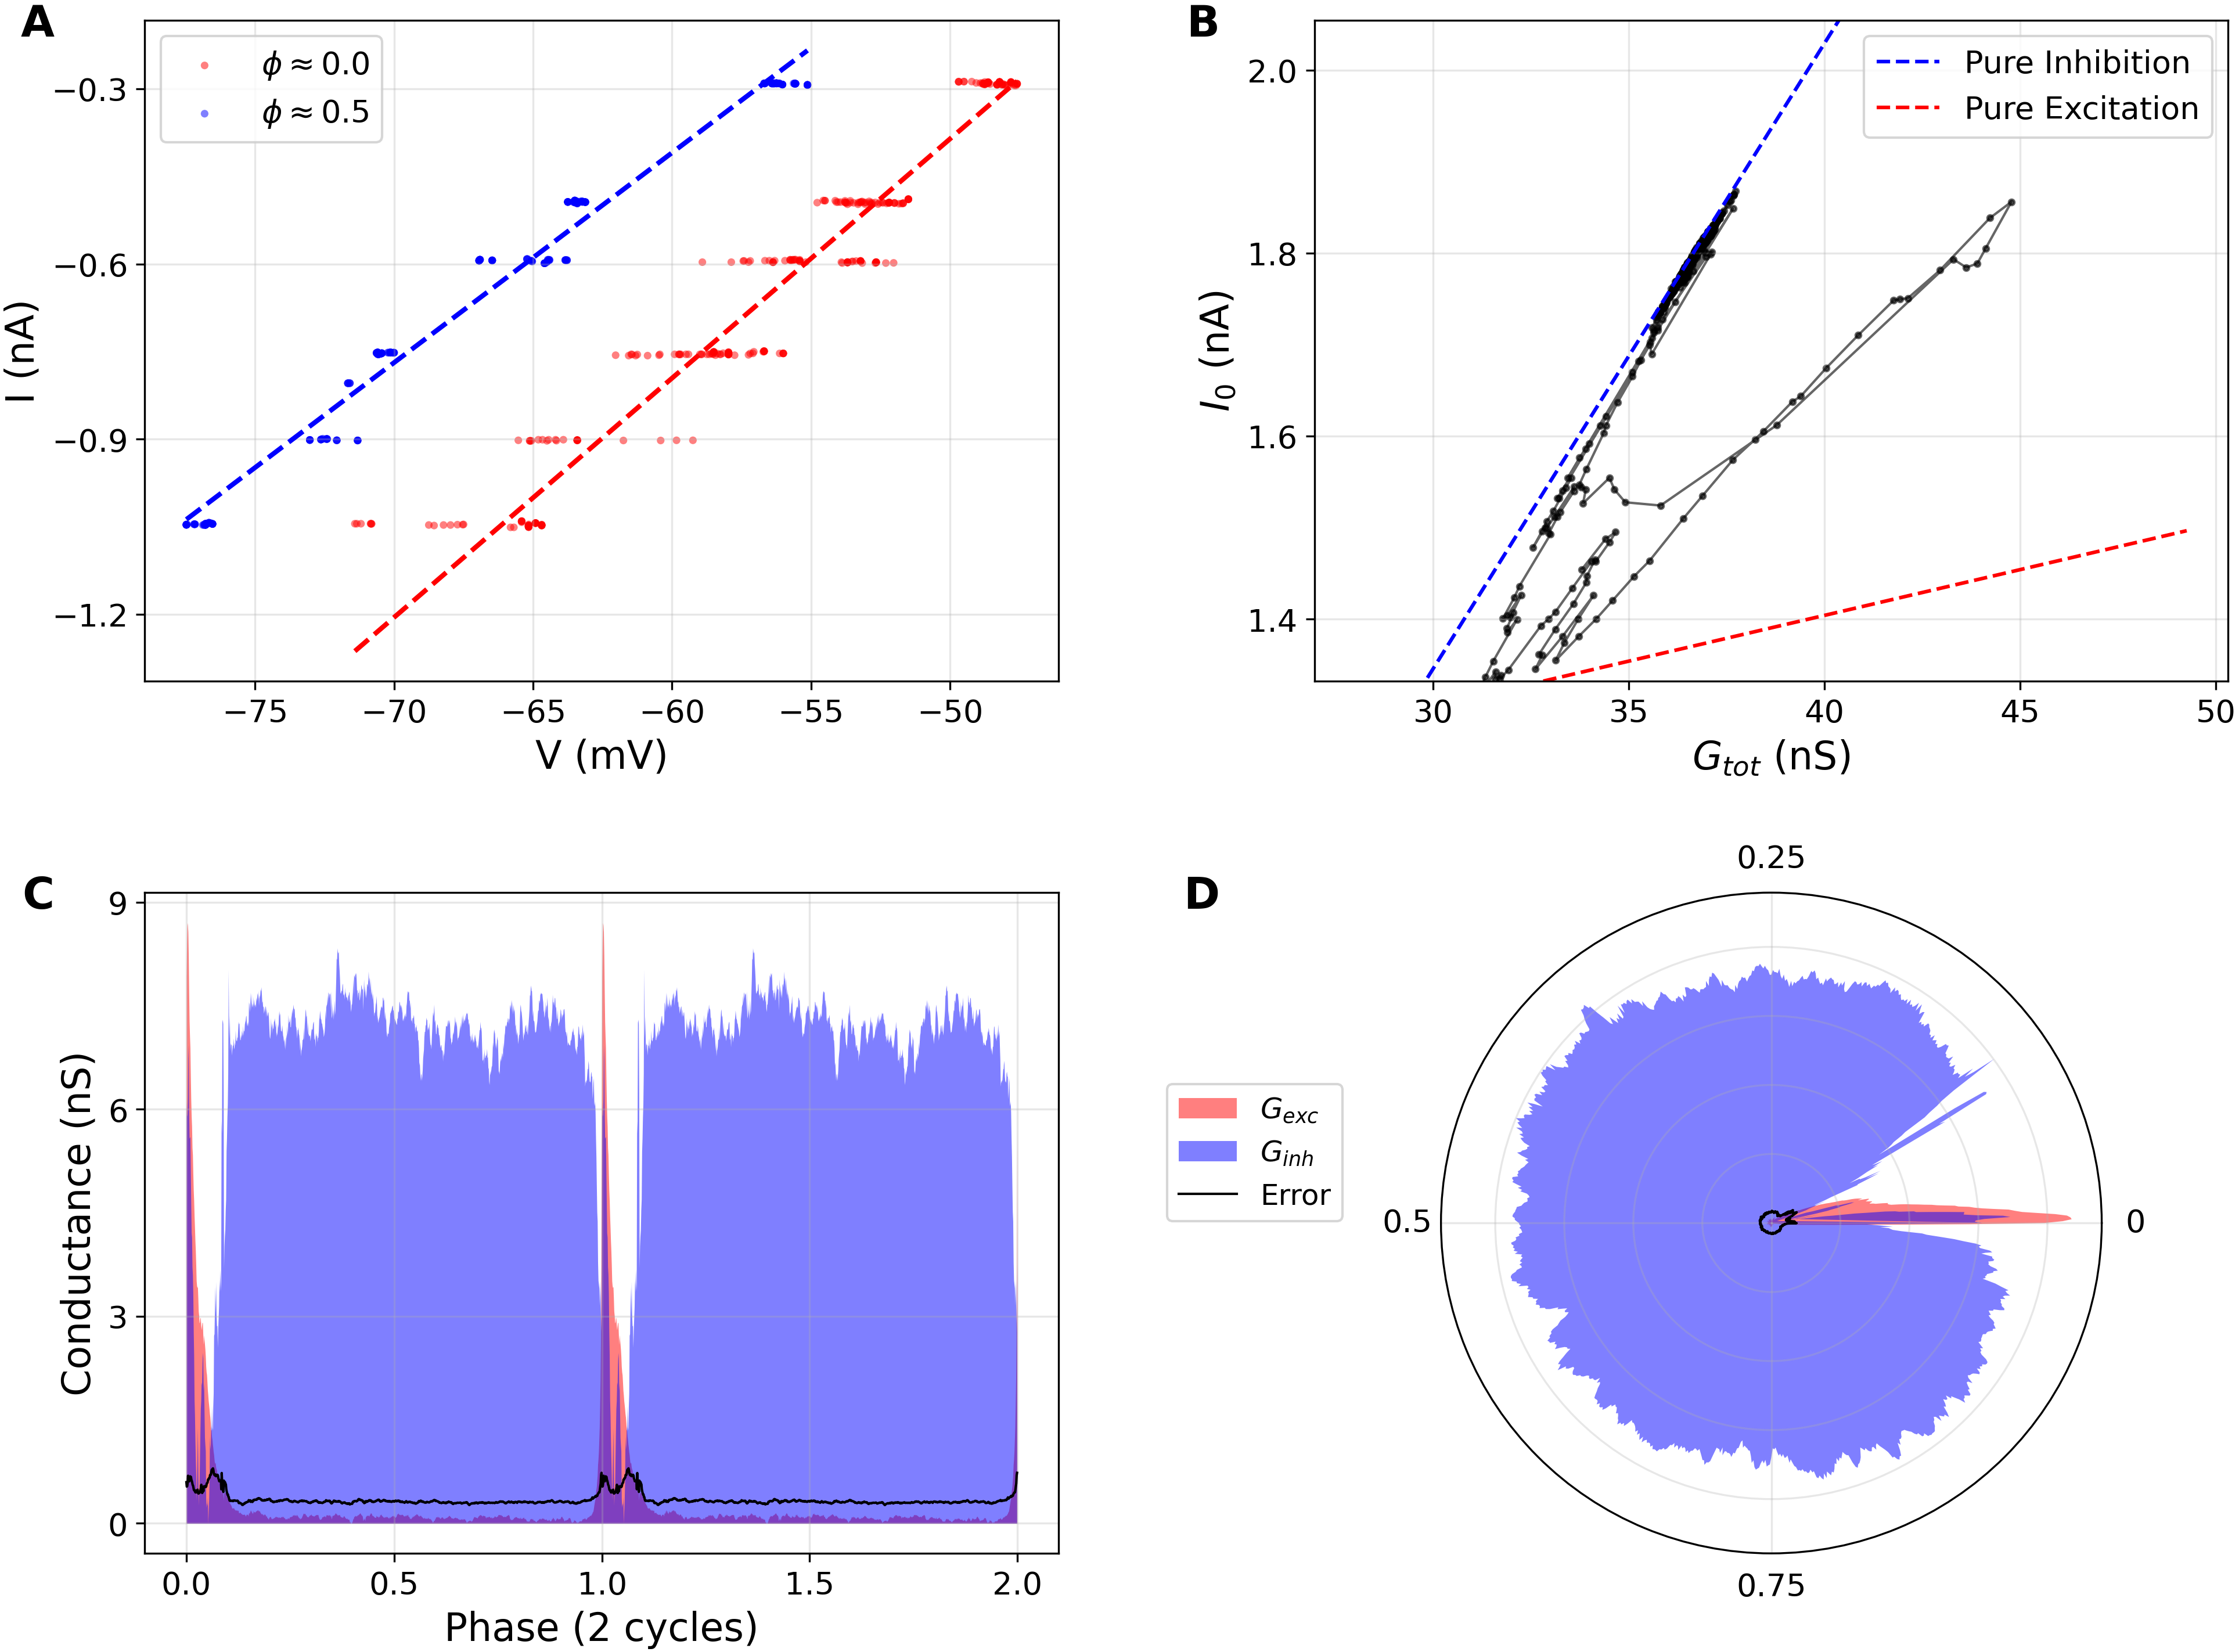
\includegraphics[width=\textwidth]{figures/figure1_method.png}
\caption{Geometric conductance inference workflow. \textbf{A}, representative phase-binned $I$--$V$ regressions for two phases of the respiratory cycle. \textbf{B}, wedge plot formed by the trajectory of $(G_{\mathrm{tot}}, I_0)$ across the cycle, bounded by the theoretical pure-excitation and pure-inhibition lines. \textbf{C}, reconstructed excitatory and inhibitory conductances across two normalized cycles. \textbf{D}, the same conductances shown in polar coordinates over one normalized cycle.}
\label{fig:method}
\end{figure}

\subsection{Data-driven estimation of inhibitory reversal potential}
The conductance decomposition depends critically on the inhibitory reversal potential, so treating $E_i$ as a single fixed constant would force every recording to obey the same inhibitory geometry. Instead, we estimated $E_i$ separately for each recording from the wedge plot formed by the phase-binned regression outputs $(G_{\mathrm{tot}}(\phi), I_0(\phi))$.

Figure~\ref{fig:method}B illustrates the logic of this estimate. Each point on the black trajectory corresponds to one respiratory phase bin in the $(G_{\mathrm{tot}}, I_0)$ plane. The blue dashed line is the pure-inhibition boundary, and the red dashed line is the pure-excitation boundary. If a phase contains inhibition with negligible excitation, its point lies on the blue boundary. Adding excitation moves the point into the interior of the wedge, away from that boundary, but cannot move it above the blue line because excitatory conductance is constrained to remain nonnegative. The upper envelope of the trajectory in Figure~\ref{fig:method}B therefore reflects inhibition alone. Because the slope of that upper boundary is set by $-E_i$, the wedge geometry provides a direct recording-specific estimate of inhibitory reversal potential before excitatory and inhibitory conductances are separated.

In practice, after the robust phase-binned $I$--$V$ regressions were computed, the analyzer searched for the tightest line that remained a global upper bound of all valid wedge points and took its slope as the recording-specific value of $-E_i$. The resulting $E_i$ was then used in the subsequent conductance decomposition for that recording. The analyzer was initialized with $E_e=-10$~mV and an initial inhibitory guess of $E_i=-80$~mV; if too few valid regression points were available to define a reliable boundary, the supplied inhibitory value was retained rather than forcing a geometric estimate. In the accepted data set, however, the automatic estimate was applied to all 50 included recordings. This recording-specific procedure prevented the decomposition from depending on a single assumed inhibitory reversal potential and ensured that each inferred wedge remained internally consistent with the geometry of its own regression cloud.

\subsection{Definition of inspiratory and expiratory summary metrics}
The per-bin conductance traces were next reduced to scalar metrics for population analysis. First, the medians of $G_{\mathrm{inh}}(\phi)$ and $G_{\mathrm{exc}}(\phi)$ across all valid bins were computed, together with median absolute deviations scaled to a 3$\sigma$-equivalent threshold. Any phase bin whose inhibitory or excitatory conductance lay outside this robust threshold was marked as belonging to a transient interval. The longest consecutive transient chain on the circular phase axis was then identified as the phasic respiratory event, and the complementary bins were treated as the stationary interval.

For each recording, the analyzer exported (i) the mean inhibitory and excitatory conductances over the stationary interval and (ii) the conductances in phase bin 0. Because the phase axis was reset at XII burst onset, the phase-0 conductances were used as the inspiratory summary metric, whereas the stationary-interval means were used as the expiratory/interburst metric for the bar plots and summary tables generated in this repository.

\subsection{Population statistics and outlier handling}
Population summaries were produced separately for VgluT2-I, VgluT2-E, VGAT-I, and VGAT-E recordings. After the cycle-count screen, one row per accepted recording was written to a group-specific CSV file containing the stationary means and phase-0 conductances. Outlier handling was deliberately postponed to this stage rather than applied as a strict recording-level exclusion rule.

Outliers were handled by a standard robust two-stage procedure: calculate a provisional distribution from all accepted recordings, identify extreme points using quantile-based criteria, remove those points from the summary statistics, and then recalculate the reported mean and SEM from the retained inliers. In practice, for each group and each scalar metric, quartiles were computed across recordings, the interquartile range was defined as $\mathrm{IQR}=Q_3-Q_1$, and recordings outside the standard Tukey interval
\begin{equation}
\left[Q_1 - 1.5\,\mathrm{IQR},\; Q_3 + 1.5\,\mathrm{IQR}\right]
\end{equation}
were labeled as outliers. Mean and SEM were then recomputed from the retained inliers only. Outliers were still displayed in the summary figure as separate markers but were not included in the reported group means or SEM values. This is a standard accepted way to summarize small, heterogeneous experimental data sets while limiting the influence of rare extreme values. We adopted this two-stage strategy because the slice data set contains recordings with limited command span or weaker reference signals that would be lost under rigid step-count criteria even though their reconstructed conductances fall well within the physiological distribution of the corresponding population.

\subsection{Software implementation}
All analyses in this repository are reproducible from the project Makefile. Conductance inference is implemented in \texttt{src/trace\_analyzer.cpp}; phase aggregation, outlier filtering, table generation, and figure production are handled by the Python scripts in \texttt{scripts/}. The standalone methods draft presented here is therefore synchronized with the actual analysis code rather than being a prose-only summary of a previous manuscript version.

\bibliography{references}

\end{document}
